

\chapter{Methodology}

To calculate the flux of fireballs from our D6 AllSky Camera, we need to find the total observation area, time, and the total number of events.
In this section, we begin by describing in detail our methods for finding each of these properties.
Some time will be spend discussing obstacles such as camera fish-eye effect and cloud interference.  
Additionally, we will delve into the structure of our database: our fundamental tool for secondary statistical analysis.

\section{Calculating Total Observation Time}

Each night the D6 AllSky camera observes, a program is run on the controlling Raspberry Pi that logs important information throughout the night.
The observation log is a simple time-stamped text file that records what processes the system runs at various times in a given night.
For instance, the observation log contains when each observation run begins (when the camera is set up initially), when the camera begins its analysis, when a new event is detected, and when the analysis goes to sleep, along with potential warnings or error messages that might come up.

To calculate the total observation time, we run a Python script that searches for the time associated with the start of each new analysis.  
After this time is recorded, we continue down the list of information until we find the time associated with that observation run's end.  
By subtracting the two times, we find the total observation time for that specific night.  
Performing this same method in a loop throughout all of the nights allows us to find how much time we spent observing on a given night. 
By summing up the total time observed over each night, we can attain the total observation time over the course of our data collection period.

A depiction of a portion of an observation log and our time analysis table can be seen in Figure~\ref{obslog_time}.
Note that while the information row that contains "New Observation Run Started" sounds as if it represents the start time, we define our start time from the information row that states "A new night has arrived! Frame analysis beginning!".\comment{Should comment on why this is.}
End times are determined by the information rows labeled "Day has come.  Analysis going to sleep."

\begin{figure}[ht!]
  \centering
  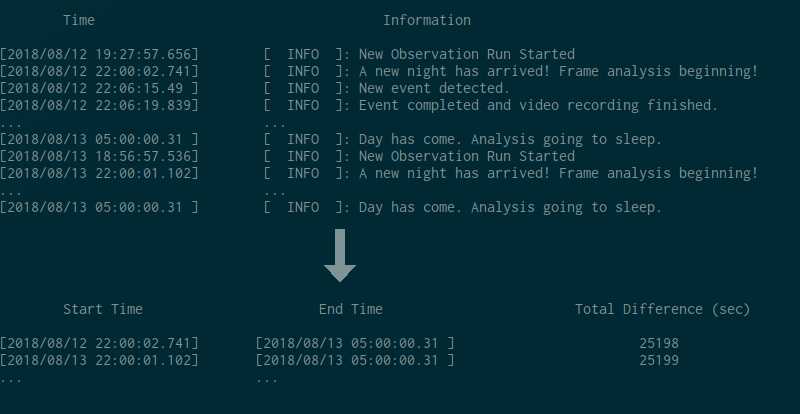
\includegraphics[scale=0.53]{images/obslog_time.png}
  \caption{An example observation log and the resulting time analysis information}
  \label{obslog_time}
\end{figure}

It is imperative that we save not only the total observing time over a given night, but also the start and end times. \comment{Is it important to comment about errors you find when doing this matching? Or if you throw away tiny portions where the camera was clearly being tested?}
This information is crucial for the next section, where we calculate the area of sky observed on a given night.

\section{Calculating Total Observation Area}

One of the most difficult problems we needed to address for this project was determining what area of the sky the D6 AllSky Camera observed each night.  
In an ideal world, our camera would be able to see all parts of the observable night sky, spanning across all horizons.  
However, due to optical limitations of our system and fisheye lens, this is not possible. 
Nevertheless, determining the flux is a primary goal of this project, and is directly dependent on observation area. As such it is vital we come up with a means to get a precise estimate\comment{This seems a bit of a paradox\ldots}. \inlinecomment{In this paragraph you were mainly focusing on the issue of us not getting the entire circle within our field-of-view, correct? Might want an image to better illustrate that.}

To make matters more complicated, while the use of a fisheye lens gets us more coverage of the sky, it also results in some distortion of the image.
These distortions generally get worse the further an object is from is from zenith (directly overhead).
An an example, imagine a square cloud located directly overhead.  
As that square drifts towards any given horizon, its size becomes smaller relative to you, the observer.\comment{Probably need more evidence or argument than this.}
The significance of this problem as related to our project stems from the fact that while $50\% $ of our camera's pixels may be covered by clouds, this doesn't necessarily mean that $50\%$ of the observable sky is covered.\comment{good, and well put.}
Therefore, we need some way of relating a given camera region to some observable distance.

To do this, we used observations of the Moon and various stars to calculate angular distance to pixel ratios for different regions of our camera.
This solution addresses the need to account for a camera fish-eye effect by assigning different fields-of-view to different pixel observational areas.
By correlating certain pixels with specific angular distances, we can analyze the available sky coverage by summing across all pixels.
To fully understand the methodology behind calculating the total observation area, one must understand how angular separation serves a role in area coverage.

\subsection{Angular Separation}

Consider two objects, both of which are visible to you, an observer.
One simple way to compare the two objects is by measuring the direct distance between them.  
An alternative way to compare the two would be to imagine two straight lines extending from your location to both objects.  
Because both lines are extending from the same location, we can calculate the associated angle between the two lines, known as the angular separation.
This angular separation may change as you move locations if the objects are nearby. However, if both objects are extremely far away, no small change in observer location will change the angular separation significantly.\comment{We use angular separation because we have no idea what radial distance separates the objects (generally). As such, we treat everything as being an equal radial distance away, and hence get the concept of the celestial sphere. And angles are a natural way to measure displacement on a sphere.}

We can apply this concept and principle to calculating angular distances between stars and other celestial objects.
By finding the angular separation across a given pixel, we attain a precise estimate\comment{this again} for angular coverage of the camera.\comment{only if we sum over all the pixels}
Assuming that the fireballs are ablating in our atmosphere at a given height, we can then apply our angular measurements to attain an observational surface area as desired.
It is easy to imagine this surface area used in flux calculations as the base of a cone, where the cone's point represents the viewer's field of view.\comment{But it is a rounded cone?}
Importantly,to calculate angular separation between objects, we need to first have a database of objects to compare.\comment{You really need a picture or pictures in this section.}

\inlinecomment{I think you need to revisit the idea that you want to use the known positions of stars and the Moon to serve as these calibration points before jumping into the next section.}
\subsection{Collecting a Star Catalog}

While the primary aim of the D6 AllSky Camera is to capture video footage of fireballs, it serves many other roles.\comment{This feels a bit awkward to me. It does these other things in an effort to better describe the population of fireballs.} 
Throughout the night, it takes several snapshots of the nights sky. 
The motivation behind this is primarily to check cloud coverage, but these images can store other important information.

Stars are visible in many D6 AllSky Camera's snapshots.  
The first step in creating a catalog of star information is recognizing stars within snapshots.  
We went about this by cleaning the image of hot spots, thresholding the image, and using the a \texttt{SimpleBlobDetector} to capture star locations.
All of these processes are coded and executed in Python.

\subsubsection{Hot Pixels and the Dark Frame}

Hot pixels are flawed pixels within a camera that always provide a significant positive photon count, even when the camera is exposed to complete darkness.
These pixels are problematic when trying to locate stars, as they don't represent any real physical object.
Fortunately, this source of error can be accounted for by taking an image while the lens of a camera is covered.  
This is called a dark frame, because the lens is not exposed to light.
Ideally the dark frame displays a black image, but most cameras will have a few hot pixels.
By subtracting this dark frame, represented by a 2-dimensional array of values ranging from $0$ to $255$, we are able to remove the hot pixel's effect from all other frames.\comment{An example would be nice.}

\subsubsection{Thresholding}

Once these hot pixels are subtracted from a given frame of interest, the next step is to enact some type of threshold.
In this case, a threshold represents a cutoff photon count\comment{Careful calling these photon counts. They are related but not directly proportional. Better to just call it pixel brightness.} for every pixel.  
If a pixel has a count that is lower than the threshold, that photon count is changed to zero, which is pure black.  
Alternatively, if a pixel has a count that is higher, the  count becomes 255, or pure white.  
Thresholding serves the important role of simplifying an image to a purely black and white, on or off type image.
It also remove some of the inherent error associated with photon counts.\comment{How are you justifying this? Or what do you mean?}
The necessary threshold for different images differed in accordance with the amount of surrounding light.
For the purposes of this project, we used an initial threshold of $140$.
If $140$ was not a sufficient threshold, this value was increased in increments of $5$ until the resulting image appeared to properly segment between open sky and clouds. 
For example, images that contained the Moon, a bright source that tends to wash out neighboring pixels, needed higher threshold values than images without.\comment{I'd like to see some images illustrating this here as well.}

\subsubsection{SimpleBlobDetector and Stellarium}

Next, we use the \texttt{SimpleBlobDetector} function from the \texttt{CV2} library to detect potential stars.
This function is able to read an image and scan for objects that meet your specified parameters.
Variable parameters include, but are not limited to, size (in pixels), circularity, convexity, and color.
In this instance, the color has a value of $255$.\comment{What about those other parameters?} 
When enacted, this function scans the picture and returns a list of detected locations centered on the object.
Using simple plotting functions, we can overlay these locations with the original image.

At this point, we have a list of potential object locations, but no foreseeable way of identifying the real ones.
As luck would have it, \textit{Stellarium}, a free astronomy software allows users to view a clear night sky from any point on earth at any time.
Additionally, this interactive software stores information about the stars' names and other important information.
By viewing \textit{Stellarium} and a D6 AllSky Snapshot and comparing the two, we are able to recognize which objects are real and which are false positives.\comment{"Why are there false positives? I thought we eliminates the hot spots?"}
Because each snapshot is labeled with the corresponding data and time, this method proved sufficient in identifying celestial objects from images.
A depiction of this process can be seen in Figure~\ref{star_recognition}.  
When comparing the two images, it should be clear that the objects numbered $17$, $16$, $19$, and $21$ correspond to Betelgeuse, Aldebaran, Capella, and Polaris. 
Also note that in the image, there are several recognized objects that don't have any celestial counterpart.
These are all false positives.
Similarly, there are cases in which the \texttt{SimpleBlobDetector} is not able to recognize an object that appears in a snapshot.
\begin{figure}[htb]
\centering
  \begin{tabular}{c|c}
    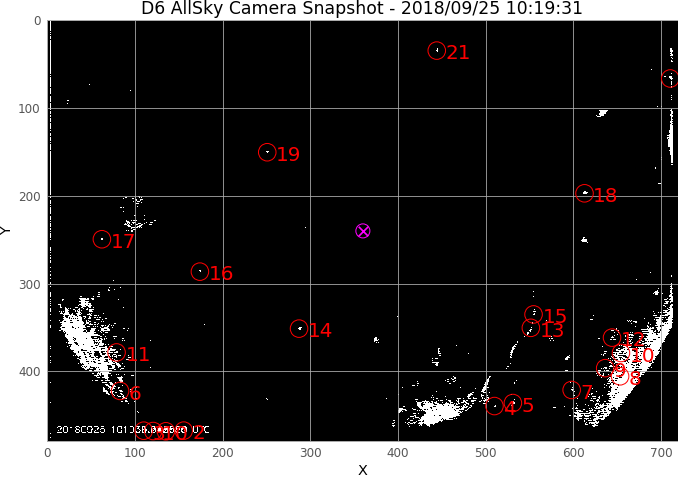
\includegraphics[width=.6\textwidth]{images/FourStarz_OneFrame.png} & 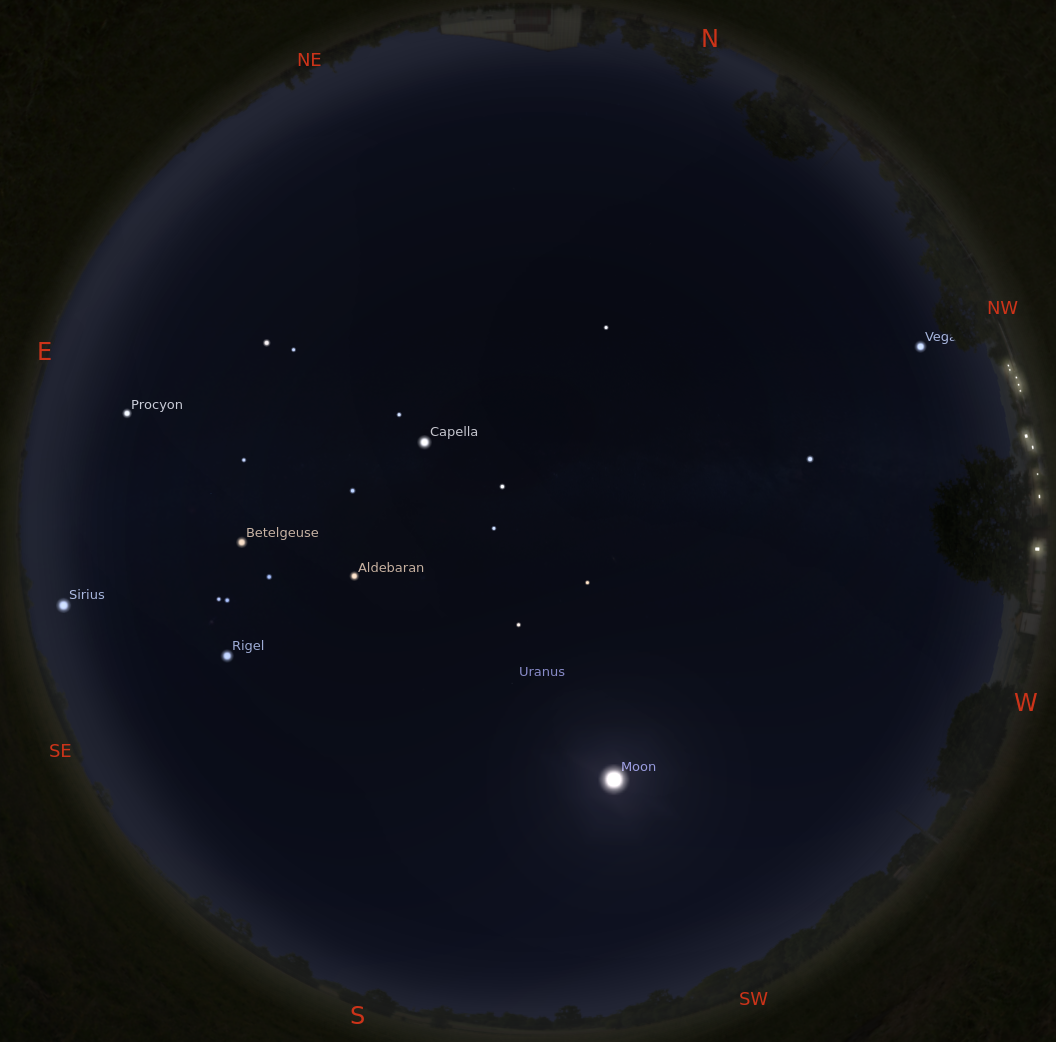
\includegraphics[width=.4\textwidth]{images/zoom_stellarium.png}
  \end{tabular}
  \caption{A D6 AllSky snapshot (left) alongside a Stellarium display (right)\inlinecomment{Please fix this image so the dark regions of the images align! Also, you need a much more robust caption explaining what is happening in each image. And you might want to zoom into Stellarium so its field-of-view roughly matches that of the image?}}
  \label{star_recognition}
\end{figure}

Once an object in a given frame is matched to a name, we used the coding library \texttt{Vizier}\comment{I'm actually not familiar with this. Is this a standard Python library or part of AstroPy?} to automatically look up the star's right ascension, declination, V-magnitude, azimuth, and elevation.  
This, combined with the star's pixel location, time, and reference file name\comment{What is this ``reference file name''?}, was added to our star catalog as a singular data row.

\subsubsection{Azimuth and Elevation}

Each star has several inherent properties such as magnitude, right ascension, and declination.  
The later two represent coordinates that locate a star on the celestial sphere.  
Other properties, such as a star's azimuth and elevation change over time and vary dependent on the observers location.  
These two properties indicate a star's position in the sky relative to an observer and act similarly to spherical coordinates.\comment{You really should comment or provide an image of what each one measures!}

Through finding the azimuth and elevation of a star, we can assign a star a 3-D coordinate value that lays on a unit sphere.  
Wwe can then calculate the angular separation between two 3-D coordinates by taking advantage of properties of the dot product:

$$ \vec{A} \cdot \vec{B} = |\vec{A}||\vec{B}| \cos{(\theta)} $$

where $\theta$ represents the angular separation between the two unit vectors.  
Because we know that both vectors representing star locations will fall on a unit sphere, their magnitude is $1$.
Using this knowledge, we may transform the above equation to:

$$ \theta = \arccos{(\vec{A} \cdot \vec{B})} $$

Given this formula along with information stored in the star catalog, we are able to calculate angular distance per pixel across different regions of the camera frame.\comment{Whoa, this is a jump. With this you can just calculate the angular separation between two points that we happen to see in our image.}


\subsection{Calculating Angular Areas}

The D6 AllSky camera is a versatile system and it's orientation can change slightly from night to night.
Because of this, there are several considerations that must be accounted for when calculating angular distance per pixel across different camera regions.
For example, if pixel $(10,10)$ has an angular separation per pixel of $0.10$ one night, if the camera rotates by $45 \deg$ we may read a different angular separation per pixel at that location. \comment{Should we though? Wouldn't the argument be that the camera should at least be rotationally symmetric?}
This is because the pixels may be representing a different area of sky upon rotation.
We have developed a method to account for this consideration.

\subsubsection{Comparing Objects from the same Night}

The star catalog stores information about celestial objects over the course of all observations.
Using constraints from the Time Analysis information (start time, end time, time elapsed), we can isolate rows within the star catalog from a specific night.  
After creating this subsection, we can then use our described method to calculate the angular separation per pixel for every combination of two objects.\comment{I'm confused. I don't feel like you have made clear how this angular separation per pixel is calculated yet?}
One might question where the data behind this angular distance per pixel should be located.
After all, there are two different object locations used to calculate the value.
Our strategy was to locate the point in between the two objects.  
Figure~\ref{starcombos} depicts these combinations along with the locations of the angular separation per pixel represented as white dots.

\begin{figure}[ht!]
  \centering
  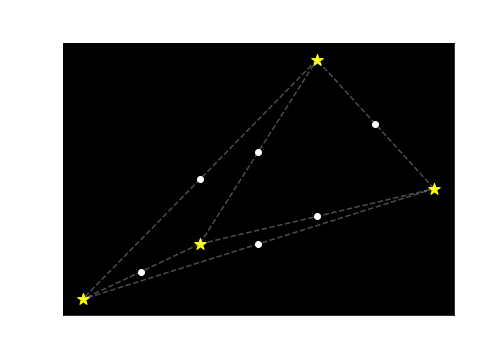
\includegraphics[scale=0.70]{images/star_combinations.png}
  \caption{A simplified depiction of angular distance per pixel locations\inlinecomment{Clarify what you mean by this.} (white dots) given a set of objects (yellow stars).}
  \label{starcombos}
\end{figure}

Figure~\ref{starcombos} gives a general depiction of our method on a much smaller scale.
Note that when comparing objects from this subsection of the star catalog, we are not limited to only comparing different stars.
As an object moves throughout the night sky, its azimuth and elevation change along with its pixel location.
We can thus treat each individual observation as a unique object, even comparing between the same object at different times throughout the night.
This creates many more combinations than if we were to only consider unique stars.

After calculating all potential angular separation per pixel values alongside their location information, we may move on to calculating average angular separation per pixel in different camera regions.
For the sake of simplicity and practicality, we split up our $720 \times 480$ pixel camera frame into $40 \times 40$ pixel squares.\comment{From a coding point of view, this wasn't really necessary. Why did we really do it?}
All angular separation per pixel measurements located inside a given square were averaged over to determine that square's value.
% Delete this picture and following sentence.  Replace with a more descriptive picture of the process, not the results.  Save for data section!
Figure~\ref{colorful2} shows the resulting average angular separation per pixel for different squares in our camera frame.\comment{Given your comment in the code. Is this the final version or the version that still needs fixed?}

\begin{figure}[ht!]
  \centering
  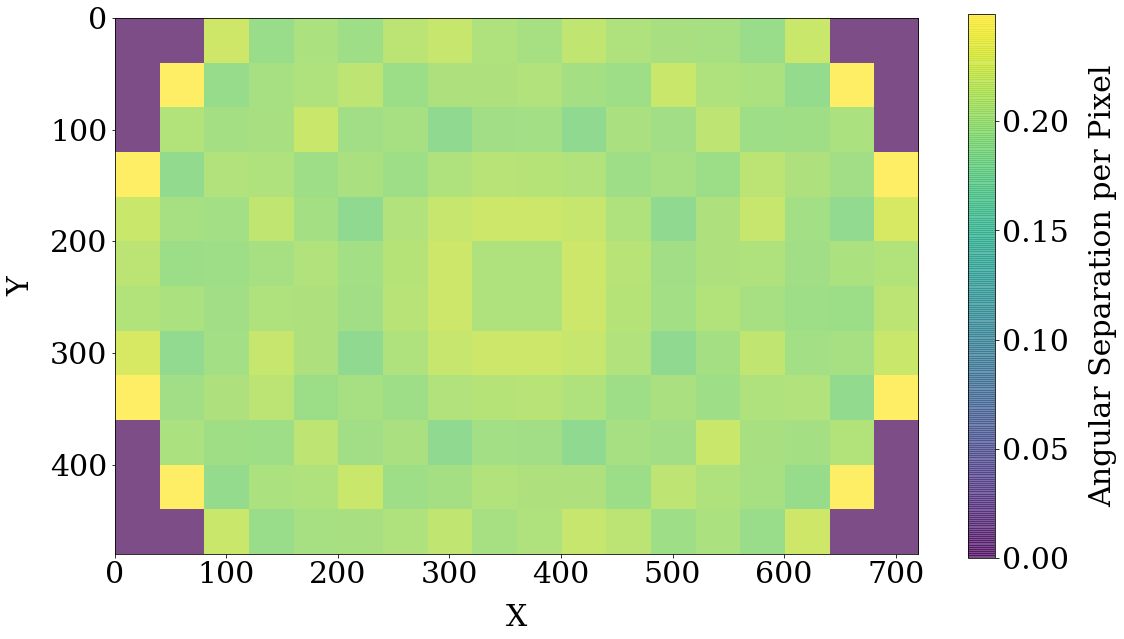
\includegraphics[scale=0.35]{images/boxes_colored.png}
  \caption{Average angular separation per pixel for different camera regions. \inlinecomment{Again, you need more robust figure captions. Also, did you ever talk about rotating the points?}}
  \label{colorful2}
\end{figure}


\section{Calculating Cloud Coverage}

The D6 AllSky Camera does not always remain outside.
For the protection of the system as well as for saving power purposes, the camera is only placed outside during nights where observation conditions are promising.\comment{That shouldn't remain that way forever though. The intent is clearly to have it outside all the time in the end.}
Some nights, the sky is clear throughout the entire night, while others are partially cloudy.\comment{Actually, given the direction you went with this, why even mention the above?}
Because we cannot see or properly analyze fireball events that happen behind clouds, we cannot count cloudy regions as observable areas.
As mentioned previously, the D6 AllSky Camera takes several snapshots of the night sky systematically throughout an observing session.
Specifically, it currently takes images every $30$ minutes.
By using thresholding, we have seen how we can determine which pixels qualify as not observable areas.
The threshold value that we used in this step was a photon value of $90$.\comment{Why does this threshold differ from the one earlier?}

Unfortunately, some pixels that fall within a broad cloud area are not recognized through this process.
The solution to this problem lies in the \texttt{CV2} functions \texttt{MORPH\_CLOSE} and \texttt{MORPH\_ERODE}.\comment{These are more any binary image functions that CV2 specific}
The first of these functions fills in regions of empty space that are next to filled in space.
This is helpful in closing gaps between pixels that represent clouds.
However, because the edges of the clouds are expanded in this process, we must subsequently perform a \texttt{MORPH\_ERODE} that works in the opposite fashion.
Once a hole is completely closed, there is no space within a cloud for the eroding function to open up, hence providing a satisfying answer to the cloud predicament.\comment{You should reference the image earlier for a visual to better understand what you are trying to eliminate.}

After this successful threshold and subsequent closing/eroding process is complete, the next step is implementing the relationships between pixels and angular distance as seen in Figure~\ref{colorful2}.
By assigning the correct regional angular separation per pixel value to each pixel within a cloud, we are able to estimate the angular area that cloud covers.
Figure~\ref{colorclouds} shows the processes taken in calculating the area occupied by clouds.
Note that both a filling and eroding function was used to attain the lower left image.
The observable area during that time is the cloud coverage subtracted from the total observation area.


\begin{figure}[ht!]
  \centering
  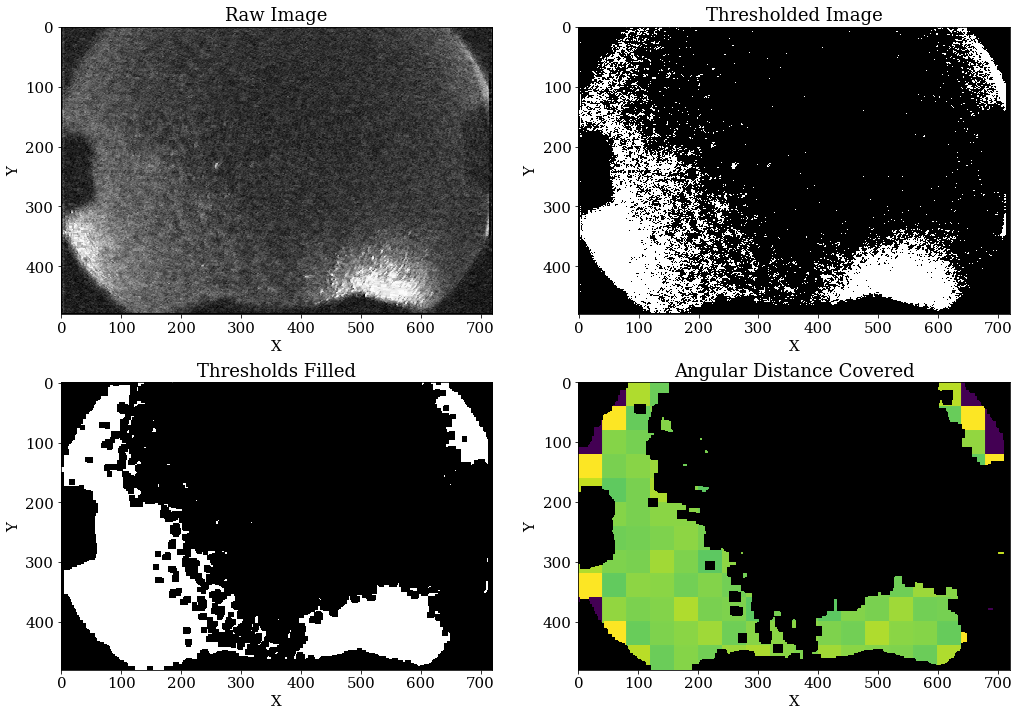
\includegraphics[scale=0.4]{images/Cloud_analysis.png}
  \caption{The processes behind determining the area of cloud coverage.\inlinecomment{Way more robust caption. This is arguably the most important image of your analysis section. Don't chince out on it!}}
  \label{colorclouds}
\end{figure}

This process is performed for each snapshot.
In creating our average area observed calculations, we assume that the sky retains that same amount of cloud coverage for the $15$ minutes prior to and $15$ minutes after the snapshot.
While this isn't precise down to the exact minute, over many observations, the number of over-estimations and under-estimations should average out and yield an accurate observational area.























 
